\documentclass{tufte-handout}

\title{z-tests and t-tests}

%\author[The Tufte-LaTeX Developers]{The Tufte-\LaTeX\ Developers}

\date{} % without \date command, current date is supplied


\usepackage{graphicx} % allow embedded images
  \setkeys{Gin}{width=\linewidth,totalheight=\textheight,keepaspectratio}
  \graphicspath{{graphics/}} % set of paths to search for images
\usepackage{amsmath}  % extended mathematics
\usepackage{booktabs} % book-quality tables
\usepackage{units}    % non-stacked fractions and better unit spacing
\usepackage{multicol} % multiple column layout facilities
\usepackage{lipsum}   % filler text
\usepackage{fancyvrb} % extended verbatim environments
  \fvset{fontsize=\normalsize}% default font size for fancy-verbatim environments

\usepackage{pgfplots}
\pgfplotsset{compat=1.12}

% Standardize command font styles and environments
\newcommand{\doccmd}[1]{\texttt{\textbackslash#1}}% command name -- adds backslash automatically
\newcommand{\docopt}[1]{\ensuremath{\langle}\textrm{\textit{#1}}\ensuremath{\rangle}}% optional command argument
\newcommand{\docarg}[1]{\textrm{\textit{#1}}}% (required) command argument
\newcommand{\docenv}[1]{\textsf{#1}}% environment name
\newcommand{\docpkg}[1]{\texttt{#1}}% package name
\newcommand{\doccls}[1]{\texttt{#1}}% document class name
\newcommand{\docclsopt}[1]{\texttt{#1}}% document class option name
\newenvironment{docspec}{\begin{quote}\noindent}{\end{quote}}% command specification environment


\begin{document}

\maketitle% this prints the handout title, author, and date


%\printclassoptions

\section{z-test (One-sample location test)}

\begin{marginfigure}
  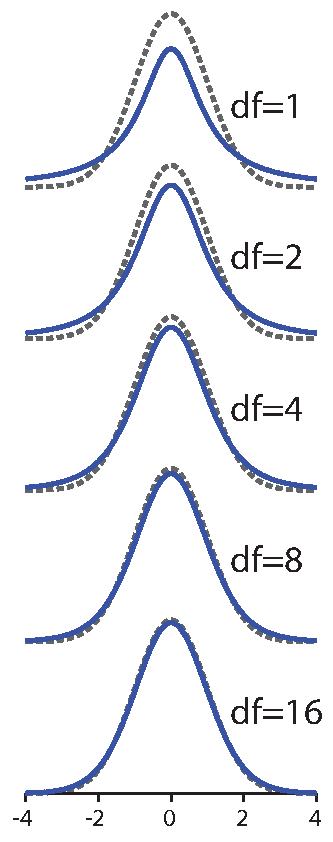
\includegraphics[width=\linewidth]{images/handout3_t_vs_norm}%
  \label{fig:fullfig}%
  \setfloatalignment{t}
  \caption{Comparison of the t-distribution (solid line) and standard normal distribution (dashed) as the degrees of freedom ($df$) increase.}
\end{marginfigure}

The goal of the one-sample z-test is to determine whether a sample mean ($\bar{X}$) shows a statistically significant difference from a known/hypothesized constant ($\mu$) when the standard deviation of the population ($\sigma$) is \emph{known}. In this case, the test statistic $z=\frac{\bar{X}-\mu}{\sigma/\sqrt{n}}$  follows a standard normal distribution, and we can quantify effect size using Cohen's $d=\frac{\bar{X}-\mu}{\sigma}$.


\section{One-sample t-test}

The goal of the one-sample t-test is to determine whether a sample mean ($\bar{X}$) shows a statistically significant difference from a known/hypothesized constant ($\mu$) when the standard deviation of the population ($\sigma$) is \emph{unknown}. Here we estimate $\sigma$ with the sample standard deviation ($s$).

The main difference between the one-sample z-test and one-sample t-test is that estimating the variance has the effect of spreading out the null distribution a little beyond what it would be if $\sigma$ were known. The effect is pronounced at small sample sizes, but with larger $n$, the difference between the normal and the t-distribution is really not very important.

Here the test statistic $t=\frac{\bar{X}-\mu}{s/\sqrt{n}}$ follows a t-distribution with $df=n-1$. To quantify effect size we can use Cohen's $d=\frac{\bar{X}-\mu}{s}$, and confidence intervals can be found using $\mu=\bar{X}\pm t_cs/\sqrt{n}$  where $t_c$  is a critical value of the t-distribution. If we want 95$\%$ confidence intervals, for instance, we can use the t-table and find the $t_c$ corresponding to a two-tailed test with $df=n-1$  and $\alpha=0.05$.

\section{Paired-sample t-test}
In a within-subjects or matched experimental design, rather than comparing a group mean to a constant, we instead want to determine whether the sample means for two measurements (from the same subjects) show a statistically significant difference. Here use a test statistic very similar to the one-sample t-test, but the trick is to first compute difference scores $X_D=X_2-X_1$  for each score pair (e.g. the difference between pre- and post-test for each participant).

Here the test statistic $t=\frac{\bar{X}_D-\mu_D}{s_D/\sqrt{n}}$ follows a t-distribution with $df=n-1$  where $\bar{X}_D$  is the mean of the difference scores and $s_D$  is the standard deviation of the difference scores. Note that $n$  here is the number of differences \emph{not} the total number of scores ($n_1+n_2$). In almost all cases, we will set $\mu_D=0$, meaning that the "expected difference under the null hypothesis" is zero. Similar to the one-sample t-test, Cohen's d is $d=\frac{\bar{X}_D-\mu_D}{s_D}$  and confidence intervals are given by  $\mu_D=\bar{X}_D\pm t_c s_D / \sqrt{n}$.


\begin{marginfigure}
  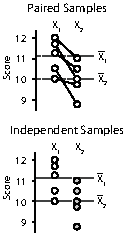
\includegraphics[width=\linewidth]{images/handout3_paired_vs_indep}%
  \label{fig:fullfig}%
  \setfloatalignment{b}
  \caption{Paired vs Independent samples. Within-subjects designs are often preffered because they allow us to control for individual differences. Even though the differences between the means are identical, only the paired data shows a significant difference. When the data is paired, it's clear that there is a consistent decrease from condition 1 to condition 2 ($s_D<s_p$).}
\end{marginfigure}

\section{Independent-sample t-test}

Finally, in a between-subjects (independent measures) experimental design we want to determine whether the sample means for two independent groups show a statistically significant difference. Here we cannot use differences between pairs of scores. Since these are completely different participants, any pairing would be arbitrary. Instead we need to calculate a statistic that takes the means and variances of each group into account.

There are two, slightly different, approaches to independent sample t-tests: \emph{Student's t-test} assumes that the two groups have equal variances, while \emph{Welch's t-test} assumes that the two groups have unequal variances. For most applications it is better to use Welch's t-test, which has the test statistic

\begin{equation*}
t=\frac{(\bar{X}_1-\bar{X}_2)-(\mu_1-\mu_2)}{\sqrt{\frac{s_1^2}{n_1}+\frac{s_2^2}{n_2}}}
\end{equation*}

where $X_1$ and $X_2$ denote the means from groups $1$ and $2$ and $s_1^2$ and $s_2^2$ denote the variances. Welch's t-statistic follows a t-distribution with a somewhat complicated $df$. Software will give you the exact values, but when working t-tests by hand you can assume that the $df$ is the smaller of $n_1-1$ and $n_2-1$.

The confidence intervals are given by
\begin{equation*}
(\mu_1-\mu_2)=(\bar{X}_1-\bar{X}_2) \pm t_c \sqrt{\frac{s_1^2}{n_1}+\frac{s_2^2}{n_2}}.
\end{equation*}

However, for Cohen's d, in this case, $d=\frac{(\bar{X}_1-\bar{X}_2)-(\mu_1-\mu_2)}{s_p}$, we need to calculate a \emph{pooled} standard deviation

\begin{equation*}
s_p=\sqrt{\frac{SS_1+SS_2}{n_1+n_2-2}}
\end{equation*}

where $SS_1=\sum{(X-\bar{X}_1)^2}$ is the sum of squares for group 1, which has sample size $n_1$, and $SS_2=\sum{(X-\bar{X}_2)^2}$  is the sum of squares for group 2, which has sample size $n_2$. As with the paired t-test, in almost all cases we set $\mu_1-\mu_2 = 0$, meaning that the "expected difference under the null hypothesis" is zero.

\marginnote[-7.0em]{Note: Welch's t-test assumes that the two groups have unequal variances. Student's t-test, which is often also returned by software, assumes that variances are equal. Unless you have a good reason to assume that variances are equal it is typically better to use Welch's method. Additionally, keep in mind that all z-tests and t-tests make the assumption that the population is normally distributed. For sufficiently large $n$ this is not an issue, since the distribution of sample means becomes normal, but for small sample sizes it can lead to problems.}


\section{Paired Sample t-test Example}

\begin{margintable}[80pt]
  \setfloatalignment{t}
  \fontfamily{ppl}\selectfont
  \begin{tabular}{rrr}
    \toprule
    Subject & No Imagery & Imagery\\
    \midrule
1&	5&	11\\
2&	6&	6\\
3&	5&	4\\
4&	9&	13\\
5&	8&	11\\
6&	8&	7\\
7&	6&	11\\
8&	7&	14\\
9&	9&	13\\
    \bottomrule
  \end{tabular}
  \label{tab:normaltab}
\end{margintable}


Dr. Smith is a cognitive psychologist interested in the role of imagery on memory. He decides to conduct a counter-balanced repeated-measures experiment where, in one condition, participants are asked to memorize a list of words without explicit instructions, and, in a second condition, using a different list of words, participants are instructed to think of a picture of each individual word in the list. He records how many words subjects can recall under the two conditions. Data from 9 subjects is shown in the table at right.

\begin{description}
\item[1.] State the null and alternate hypotheses, 
\item[2.] Calculate the appropriate test statistic, 
\item[3.] Find the critical value 
\item[4.] State your conclusion about the null hypothesis 
\item[5.] How large is the effect size in the study?
\end{description}

Note: all assumptions are satisfied, use alpha = .05, two-tailed test.

\pagebreak
\section{Independent Sample t-test Example}

\begin{margintable}[20pt]
  \setfloatalignment{t}
  \fontfamily{ppl}\selectfont
  \begin{tabular}{rr}
    \toprule
No Imagery & Imagery\\
    \midrule
8&	3\\
2&	7\\
4&	7\\
5&	3\\
6&	8\\
3&	6\\
5&	6\\
7&	8\\
    \bottomrule
  \end{tabular}
  \label{tab:normaltab}
\end{margintable}

After analyzing the data from his first experiment, Dr. Smith decides that there may have been practice effects in his within-subjects design. He decides to conduct a second experiment using completely separate groups. Participants are now randomly assigned to one of two groups: in group one, participants are asked to memorize a list of words without explicit instructions, and, in group two, using the same list of words, participants are instructed to think of a picture of each individual word in the list. He records how many words subjects can recall under the two conditions. Data from 16 subjects is shown in the table at right.

\begin{description}
\item[1.] State the null and alternate hypotheses, 
\item[2.] Calculate the appropriate test statistic, 
\item[3.] Find the critical value 
\item[4.] State your conclusion about the null hypothesis 
\item[5.] How large is the effect size in the study?
\end{description}

Note: all assumptions are satisfied, use alpha = .05, two-tailed test.

\pagebreak

\section{Paired Sample t-test Example - Solution}
\begin{fullwidth}
\begin{description}
\item[1.] $H_0$: $\mu_D=0$ (there is no difference between the imagery and no imagery condition)\\
$H_A$: $\mu_D\neq0$ (there is a difference between the conditions)

\item[2.] We're using a paired t-test. In this case, the test statistic
\begin{equation*}
t=\frac{\bar{X}_D-\mu_D}{s_D/\sqrt{n}}
\end{equation*}
follows a t-distribution with $df=n-1$ where $\bar{X}_D$ is the mean of the difference scores and $s_D$ is the standard deviation of the difference scores. After calculating the individual differences

\begin{table}
  \centering
  \fontfamily{ppl}\selectfont
  \begin{tabular}{rrrr}
    \toprule
Subject&	No Imagery&	Imagery&	$X_D$\\
    \midrule
1&	5&	11&	6\\
2&	6&	6&	0\\
3&	5&	4&	-1\\
4&	9&	13&	4\\
5&	8&	11&	3\\
6&	8&	7&	-1\\
7&	6&	11&	5\\
8&	7&	14&	7\\
9&	9&	13&	4\\
    \bottomrule
&&&$\bar{X}_D=3$\\
&&&$s_D=3$\\
    \bottomrule
  \end{tabular}
  \label{tab:normaltab}
  %\zsavepos{pos:normaltab}
\end{table}
\vspace{20pt}
we find  $\bar{X}_D=3$ and  $s_D=3$. Our null hypothesis is that $\mu_D=0$ so $t=\frac{3-0}{3/\sqrt{9}}=3$.

\item[3.] Using the t-table we look up the critical value. Look for the row for $df=n-1=9-1=8$ and the column for the $\alpha=0.05$ two-tailed, where we find $t_c=2.306$.
\item[4.] Since $t>t_c$, we reject the null hypothesis, and conclude that the groups have a statistically significant difference.
\item[5.]For the paired t-test the effect size is given by $d=\frac{\bar{X}_D-\mu_D}{s_D}$. Plugging in our previous values we get $d=3/3 = 1.0$.
\end{description}
\end{fullwidth}

\pagebreak

\section{Independent Sample t-test Example - Solution}

\begin{fullwidth}
\begin{description}
\item[1.] $H_0$: $\mu_1=\mu_2$ (there is no difference between the imagery and no imagery condition)\\
$H_A$: $\mu_1\neq \mu_2$ (there is a difference between the conditions)

\item[2.] We're using a independent sample t-test. In this case, the test statistic
\begin{equation*}
t=\frac{(\bar{X}_1-\bar{X}_2)-(\mu_1-\mu_2)}{\sqrt{\frac{s_1^2}{n_1} + \frac{s_2^2}{n_2}}}
\end{equation*}

follows a t-distribution with  $df \approx min(n_1-1,n_2-1)$. First, let's find the means and variances for the two groups

\begin{table}
  \centering
  \fontfamily{ppl}\selectfont
  \begin{tabular}{rr}
    \toprule
No Imagery & Imagery\\
    \midrule
8&	3\\
2&	7\\
4&	7\\
5&	3\\
6&	8\\
3&	6\\
5&	6\\
7&	8\\
    \bottomrule
$\bar{X}_1=5$& $\bar{X}_2=6$\\
$s_1^2=4$& $s_2^2=4$\\
$n_1=8$& $n_2=8$\\
    \bottomrule
  \end{tabular}
  \label{tab:normaltab}
  %\zsavepos{pos:normaltab}
\end{table}
\vspace{20pt}
Since our null hypothesis assumes that $\mu_1=\mu_2$ we have $t=\frac{(5-6)-0}{\sqrt{4/8+4/8}}=-1$

\item[3.] Using the t-table we look up the critical value. Look for the row for $df=min(n_1-1,n_2-1)=7$ and the column for the $\alpha=0.05$ two-tailed, where we find $t_c=2.36$.

\item[4.] Since $-2.36<t<2.36$, we fail to reject the null hypothesis, and cannot conclude that the groups are different.

\item[5.]For the independent samples t-test the effect size is given by

\begin{equation*}
d=\frac{(\bar{X}_1-\bar{X}_2)-(\mu_1-\mu_2)}{s_p}.
\end{equation*}

The pooled variance is given by
\begin{equation*}
s_p^2=\frac{SS_1+SS_2}{df_1+df_2}=\frac{28+28}{7+7}=4
\end{equation*}

Then plugging in our previous values we get $d=\frac{(5-6)-0}{\sqrt{4}}=0.5$.
\end{description}
\end{fullwidth}
\end{document}
